\section{Causal Reasoning for Systems}
\label{sec:causalreasoning}

% We define some frequently used terms in this paper.

% \noindent$\bullet$ {\it Configuration parameter} $c$: Is a configurable option offered by the software system (\eg, \texttt{tf.set\_memory\_growth()} in tensorflow that determines GPU usage scaling) or the hardware platform (\eg, \texttt{FAN\_MODE} in \xavier to control the fan speed). Each configuration may be a continuous value, a set of discrete values, or a boolean variable. 

% \noindent$\bullet$ \textit{Configuration}~$\mathcal{C}$: Is an array $[c_1, \ldots, c_N]$ of size $N$ where each element $c_i$ is a configuration parameter $c$ and $N$ is the number of configurable parameters.  

% \noindent$\bullet$ Configuration {\em space} $\zeta$: Are space of all valid configurations for a given software system and the hardware platform. Given a configuration $\mathcal{C}$, if each configuration $c\in\mathcal{C}$ can take an average of $M$ possible values, then the size of configuration space $\zeta$ is approximately equal to $M^N$. 

% \noindent$\bullet$ {\it Performance Objective} $Y_i$: Is a measurement that quantifies the behavior of a software system deployed on a hardware platform operating under a configuration $\mathcal{C}$. The performance of deployment may be measured in multiple ways such as inference time (\ie, latency), energy consumption, or heat dissipation. 

% % \begin{wrapfigure}[17]{R}{0.5\linewidth}
% %     \centering
% %     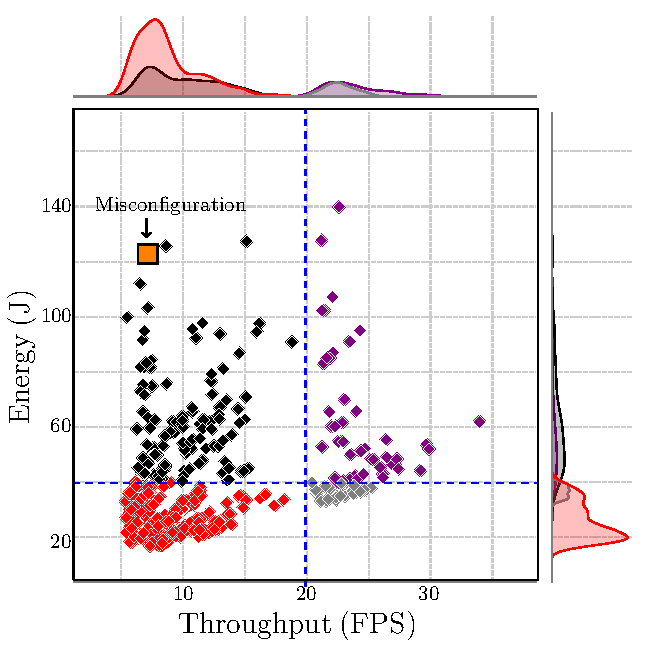
\includegraphics[width=\linewidth]{fig__spread.pdf}
% %     \caption{\small An example of multi-objective non-functional faults.}
% %     \label{fig:faults_eg}
% % \end{wrapfigure}

% \noindent$\bullet$ \textit{non-functional fault} $Y_i^{\small {\sc fault}}$. Is an anomaly in configuration $\mathcal{C}$ that results in the performance objective taking tail values \ie, values worse than or 99.99\% of the remaining performance objectives.  %In~\fig{faults_eg}, \textbf{L} and \textbf{E} are faults in latency and energy.

% \noindent$\bullet$ \textit{Multiobjective-non-functional fault} $Y_i^{\small {\sc fault}}$. Is an non-functional fault $Y_i^{\small {\sc fault}}$ that affects more than one performance objective. In~\fig{faults_eg}, \textbf{LE} is a multi-objective non-functional fault.



% \subsection{Causal Graph Discovery}
% One of the most challenging tasks in dealing with causal models is learning their structures from observational (i.e., non-experimental) data. In this section, we provide a brief overview of the two main \textit{constraint-based} algorithms, that use statistical analysis to test the presence of conditional independence, for learning causal graphs: (1) \textbf{Causal Structure Discovery With Causal Sufficiency Assumptions.} A causal structure without feedback loops and without hidden variables (i.e., unmeasured common causes and selection biases), simply called causal sufficiency assumptions, can be visualized as a \textit{directed acyclic graph} (DAG) where the directed edges indicate direct cause-effect relationships. For this purpose, the PC algorithm proposed by \textbf{P}eter Spirtes and \textbf{C}lark Glymour \cite{sgs} can be used to learn the DAG structure from data by testing for conditional independence between various sets of variables.
% Given the results of these tests, a partially directed graph is constructed so that the Markov
% property holds and $d$-separation confirms the resulting graph mirroring those conditional independencies found in the data. The PC algorithm consists of two phases. In the first phase, an undirected graph is learned. This is known as the \textit{skeleton} of the
% causal graph. In the second phase, arrowheads are added to some of the edges where they can be inferred. The output graph may not be fully oriented and is called a \textit{pattern}. When the pattern contains undirected edges, these indicate that the data are
% consistent with models in which either orientation is possible.  (2) \textbf{Causal Structure Discovery Without Causal Sufficiency Assumptions.}
% The Fast Causal Inference (FCI) algorithm \cite{sgs} is a constraint-based algorithm that has been explicitly designed to infer conditional
% independence and causal information without assuming causal sufficiency. Similar to the PC algorithm, FCI outputs a class of causal graphs that are Markov equivalent over the measured variables. The output is a \textit{partial ancestral graph} (PAG) that represents the features common to all of the DAGs in the equivalence class. Note that, PC and FCI do not necessarily provide complete causal information because
% they output (independence) equivalence classes, i.e., a set of
% causal structures satisfying the same conditional independences. For a brief review of the computational methods for causal discovery that were developed in the past three decades see Glymour et al. \cite{glymour2019review}.

% \subsection{Mediation Analysis}
% % \subsection{Causal Inference}
% Causal calculus is a vast field of probabilistic analysis. It is the cornerstone of Judea Pearl's seminal work on causal inference []. We provide a (very) summary here. 

% \textbf{How the issues of regression-based performance models could have been avoided.} We hypothesize that the reason behind the above-mentioned issues\footnote{there are several additional examples that support the above-mentioned issues in Appendix} is the inability of correlation-based models to capture causally relevant predictors (options and their interactions) in the learned performance models. Hence, we demonstrate how the above-mentioned issues will be avoided with an approach based on causal reasoning. 

% First, we briefly introduce few important causality concepts. 


We hypothesize that the reason behind unreliable predictions and incorrect explanations of performance influence models (see \S\ref{sec:causalreasoning}) is the inability of correlation-based models to capture causally relevant predictors in the learned performance models. The theoretical and empirical results~\cite{JSVKPA:ASE17,javidian2019transfer} also show that predictive models that contain non-causal predictors, even though they might be accurate in the environment that the training data come from, such models are not typically transferable in unseen environments.

Hence, we introduce a new abstraction for performance modeling, called \emph{Causal Performance Model}, which gives us the leverage for performing causal reasoning for computer systems. In particular, we introduce the causal performance model to serve as a \emph{modeling abstraction} that allow building \emph{reusable performance models} for downstream performance tasks, including performance predictions, performance testing and debugging, performance optimization, and more importantly, it serves as a \emph{transferable model} that allow performance analyses across environments~\cite{JSVKPA:ASE17,javidian2019transfer}.

\begin{figure}[tp!]
    % \setlength{\belowcaptionskip}{-3em}
    \centering
    \includegraphics*[width=\linewidth]{CausalModelExample}
    \caption{\small {A partial causal performance model for \textsc{Deepstream} discovered in our experiments. %Gray nodes indicate configuration options, blue colored nodes indicate system events and red colored nodes indicate performance objectives.
    }}
    
    \label{fig:causal_model_example}
    \vspace{-3mm}
    % \rayb{I have questions about this figure. Let's talk in the morning}
\end{figure}

\textbf{Causal performance models}. We define a causal performance model as an instantiation of Probabilistic Graphical Models~\cite{pearl1998graphical} with new types and structural constraints to enable performance modeling and analyses. Formally, causal performance models (cf., \fig{causal_model_example}) are Directed Acyclic Graphs (DAGs)~\cite{pearl1998graphical} with (i) performance variables, (ii) functional nodes that define functional dependencies between performance variables (i.e., how variations in one or multiple variables determine variations in other variables), (iii) causal links that interconnect performance nodes with each other via functional nodes, and (iv) constraints to define assumptions we require in performance modeling (e.g., software configuration options cannot be the child node of performance objectives; or \texttt{Cache Misses} as a performance variable takes only positive integer values). In particular, we define three new variable types: (i) Software-level configuration options associated with a software component in the composed system (e.g., \texttt{Bitrate} in the decoder component of \textsc{Deepstream}), and hardware-level options (e.g., \texttt{CPU Frequency}), (ii) intermediate performance variables relating the effect of configuration options to performance objectives including middleware traces (e.g., \texttt{Context Switches}), performance events (e.g., \texttt{Cache Misses}) and (iii) end-to-end performance objectives (e.g., \texttt{Throughput}). In this paper, we characterize the functional nodes with polynomial models, because of their simplicity and their explainable nature, however, they could be characterized with any functional forms, e.g., neural networks~\cite{xia2021causal,scherrer2021learning}. We also define two specific constraints over causal performance models to characterize the assumptions in performance modeling: (i) defining variables that can be intervened (note that some performance variables can only be observed (e.g., \texttt{Cache Misses}) or in some cases where a variable can be intervened, the user may want to restrict the variability space, e.g., the cases where the user may want to use prior experience, restricting the variables that do not have a major impact to performance objectives); (ii) structural constraints, e.g., configuration options do not cause other options. Note that such constraints enable incorporating domain knowledge and enable further sparsity that facilitates learning with low sample sizes.


\textbf{How causal reasoning can fix the reliability and explainability issues in current performance analyses practices?}.
The causal performance models contain more detail than the joint distribution of all variables in the model. For example, the causal performance model in \fig{causal_model_example} encodes not only \texttt{Branch Misses} and \texttt{Throughput} readings are dependent but also that lowering \texttt{Cache Misses} causes the \texttt{Throughput} of \textsc{Deepstream} to increase and not the other way around. The arrows in causal performance models correspond to the assumed direction of causation, and the absence of an arrow represents the absence of direct causal influence between variables, including configuration options, system events, and performance objectives. The only way we can make predictions about how performance distribution changes for a system when deployed in another environment or when its workload changes are if we know how the variables are causally related. This information about causal relationships is not captured in non-causal models, such as regression-based models. %We have to introduce something more expressive than the statistical distribution based on performance data. 
Using the encoded information in causal performance models, we can benefit from analyses that are only possible when we explicitly employ causal models, in particular, interventional and counterfactual analyses~\cite{pearl2009causality, pearl2018book}. For example, imagine that in a hardware platform, we deploy the \textsc{Deepstream} and observed that the system throughput is below 30 \texttt{FPS} and \texttt{Buffer Size} as one of the configuration options was determined dynamically between 8k-20k. The system maintainers may be interested in estimating the likelihood of fixing the performance issue in a counterfactual world where the \texttt{Buffer Size} is set to a fixed value, 6k. The estimation of this counterfactual query is only possible if we have access to the underlying causal model because setting a specific option to a fixed value is an intervention as opposed to conditional observations that have been done in the traditional performance model for performance predictions.  


% Causal performance models are more fine-grained, more informative, and more reliable for performance predictions in different environments, compared to statistical regression-based performance models. 
Causal performance models are not only capable of predicting system performance in certain environments, they encode the causal structure of the underlying system performance behavior, i.e., the data-generating mechanism behind system performance. Therefore, the causal model can reliably transfer across environments~\cite{scholkopf2021toward}. To demonstrate this for causal performance models as a particular characterization of causal models, we performed a similar sensitivity analysis to regression-based models and observed that causal performance models can reliably predict performance in unseen environments (see \fig{barplot_hw_change} (b)). In addition, as opposed to performance influence models that are only capable of performance predictions, causal performance models can be used for several downstream heterogeneous performance tasks. For example, using a causal performance model, we can determine the \emph{causal effects} of configuration options on performance objectives. Using the estimated causal effects, one can determine the effect of change in a particular set of options towards performance objectives and therefore can select the options with the highest effects to fix a performance issue, i.e., bring back the performance objective that has violated a specific quality of service constraint without sacrificing other objectives. Causal performance models are also capable of predicting performance behavior by calculating conditional expectation, $E(Y|X)$, where $Y$ indicates performance objectives, e.g., throughput, and $X=x$ is the system configurations that have not been measured.


% \begin{figure}[t!]
% \small
%     % \setlength{\belowcaptionskip}{-3em}
%     \centering
%     \includegraphics*[width=\linewidth]{figures-vg/cm_barplot_hw_change.pdf}
%     \caption{\small {Causal models generalize better as the number of common terms, total terms and prediction error of the structural does not change much from source (\xavier) to target (\txtwo). The rank correlation between source and target is 0.49 (p-value=0.76).}}
%     \label{fig:deepstream_across_environments_cm}
    
%     % \rayb{\\ The font needs to be updated. The text under configuration option shows very limited options per sub-system and does not reflect the complexity}
% \end{figure}

% The main difference between performance models based on causal effects and inference of association, what we called a correlation-based approach, is that causal inference analyzes the response of an effect variable when a cause of the effect variable is changed.
% Let us use a partial causal model, see Fig.~\ref{fig:causal_model_example}, that has been learned on the DeepStream performance data. Based on the causal model, we can perform analyses not only based on observational data, similar to mainstream machine learning but also, we can benefit from analyses that are only possible when we explicitly employ causal model, in particular, interventional and counterfactual analyses~\cite{pearl2009causality, pearl2018book}. For example, imagine that in a hardware platform, we deploy the DeepStream and observed that the system throughput is below 30/s and \textsc{BufferSize} as one of the configuration options was determined dynamically between 8k-20k. The system maintained may be interested in estimating the likelihood of fixing the performance issue in a counterfactual world where the \textsc{BufferSize} is set to a fixed value, 6k. The estimation of this counterfactual query is only possible if we have access to the underlying causal model because setting a specific option to a fixed value is an intervention as opposed to conditional observations that have been done in the traditional performance model for performance predictions.  

% Accordingly, let us assume that we have gathered several samples of $\text{\cpufreq}$, $\text{\gpugrowth}$, $\text{\swapmem}$, and $\text{\texttt{Latency}}$ \etc. Say, we are interested in how \texttt{latency} behaves given \gpugrowth, then, from a causal perspective, this can be formulated in three ways: observational, interventional, and counterfactual~\cite{pearl2009causality, pearl2018book}.




% Let us assume we have adequate data and the state-of-the-art tools (say, deep networks) to fully estimate this joint distribution, or any property thereof. 
% \textbf{Observation, Intervention, and counterfactual.}
% In most typical performance analysis scenarios, we measure performance objectives, e.g., throughput ($Y$), for various system configurations (\ie, $X=x$). Given adequate \emph{observational} performance data, modern supervised machine learning models, such as non-linear regression models, can be trained on performance data and used as predictive models to estimate the performance objectives for the configurations, in the configuration space of the system, that has not been measured. Such predictive model estimates conditional probability distribution $Pr(Y~|~X=x)$. However, any regression models of these sorts are not able to capture the underlying causal relationships, and therefore, any term that appears in the performance model cannot be interpreted as if they causally have an impact on the performance behavior of the system. For instance, they may have appeared because the regression model overfitted the performance data. In addition, there is no guarantee that most of such terms appear in performance models trained on performance data measured in other environments.

% we have \textit{observed} system events variables, $E=e$, such as \textit{Cache Misses}, and                                                                 

% In order to capture causal relations, we need to \emph{intervene} upon configurable options by pinning each option to a specific value and observe performance objectives as well as intermediate system-wide events, such as \textit{Cache Misses}, to explain how configuration options causally affect performance objectives via the intermediate system event variables. Once the interventional data have been measured, we can learn a causal model, cf. Fig.~\ref{fig:causal_model_example}, which gives us leverage to calculate the causal effects of options on performance objectives. Note that such causal effect can be \emph{estimated} if we learn the underlying causal model using the observational data. 

% \textit{interventional} inference tackles a harder task of estimating the {\em effects of deliberate actions}. For example, in~\ref{fig:complex}, we measure how the distribution of \texttt{Latency} ($Y$) would change if we (artificially) intervened during the data gathering process by forcing the variable \gpugrowth (X) to take a certain value `x', \ie, $X=x$, but otherwise retain the other variables (\ie, \swapmem) as is. 

% This is done by building a causal graph, modifying them to reflect our intervention. Later, using the modified causal graph and \textit{do-calculus}~\cite{pearl2009causality} we may estimate the outcome of the artificial intervention. This is computationally efficient since we reason over existing data instead of gathering additional measurements.

% ~\rayb{this sentence is not clear. Are you taking the actual measurement or you are guessing based on observation?}.% to estimate $Pr(Y~|~do(X=x))$. 

% \noindent\textbf{Are these really different?} Yes, because $Pr\left(Y~|~X=x\right)$ uses the original population, as is, and filters it to get the sub-population where \gpugrowth is `x' (\ie, $X=x$). If $X=x$ does not exist in the population, or when the latency ($Y$) is affected by an external variable \swapmem ($Z$), the value of $Pr\left(Y~|~X=x\right)$ would be misleading. In contrast, $Pr\left(Y~|~\mathit{do}\left(X=x\right)\right)$ uses the do-calculus expression over existing data to estimate the effect of changing \gpugrowth artificially while keeping the \swapmem unchanged. This accounts for any unexpected changes to \swapmem and consequently estimates the true causal effect of \gpugrowth on latency. Such inference is impossible with traditional ML.

% to infer the value of the distribution even when $X=x$ has never been encountered before, or when there are other interacting variables to be accounted for. 

% This is different from observational inference because now we can account for the effect of other intermediate variables, \eg, \swapmem, on latency. Since \swapmem may be throttled by the \texttt{resource manager}, we can use the do-calculus expression over the existing data to estimate the effect of changing \gpugrowth artificially while keeping the \swapmem unchanged. This will help us account for any unexpected changes to \swapmem and estimate the true causal effect of \gpugrowth on latency. Such inferences are not possible with observational approaches alone.      

% \noindent\textbf{Are these really different?}~${Pr}(Y~|~do(X=x))$ is \textit{not} the same as the ordinary conditional distribution $Pr\left(Y~|~X=x\right)$. This is because $Pr\left(Y~|~X=x\right)$ takes the original population, as is, and filters it get the sub-population where $X=x$. If $X=x$ does not exist in the population, or if $Y$ is affected by another variable $Z$, the value of $Pr\left(Y~|~X=x\right)$ would be misleading. In contrast, $Pr\left(Y~|~\mathit{do}\left(X=x\right)\right)$ uses do-calculus rules~\cite{pearl2009causality} to infer the value of the distribution even when $X=x$ has never been encountered before, or when there are other interacting variables to be accounted for. 

% There are known as identifiability problems,\eg, if the cache size of the system is ``set'' to say two times larger than its current size, will the latency of the system be reduced?

% \textbf{Counterfactual Inference} 
% \begin{figure}[t!]
    % \setlength{\belowcaptionskip}{-3em}
    \centering
    \includegraphics*[width=\linewidth]{UnicornOverview}
    \caption{\small {Overview of \ourapproach}}
    \vspace{-2em}
    \label{fig:overview}
    % \rayb{I have questions about this figure. Let's talk in the morning}
\end{figure}

% In some downstream performance tasks, we need to estimate queries of the following form:
% ""\textit{Given that we observed a high latency, and given that Bitrate have been set to 1000 and given what we have observed regarding System Events such as \textit{BranchMisses} and \textit{CacheMisses}, what is the probability of \textit{Throughput} reaches the QoS level, had we set the \textit{\textsc{BufferSize}} to 6000 instead of 20000?}""
% \noindent In other words, we are interested in a scenario where:
% \bisq
% \item We \textit{hypothetically} have low latency;
% \ei 
% Conditioned on the following events:
% \bisq
% \item We \textit{actually observed} high latency;
% \item \gpugrowth was initially set to $33\%$;
% \item We \textit{hypothetically} set the new \gpugrowth to $66\%$; and
% \item Other circumstances (available \swapmem, resource load, etc) remain the same; 
% \ei

% Formally we represent this, by abusing notations, as:
% \begin{equation}
%     \label{eq:counterfact}
%     Pr(\hat{Y}=y_{low}~|~\hat{X}=0.66,~X=0.33,~Y=y_{high},~Z)
% \end{equation}
% Here, $Y$ stands for observed latency, $X$ stands for current \gpugrowth, and $Z$ stands for current \swapmem. The variables $\hat{X}\text{ and }\hat{Y}$ are as yet unobserved (or hypothetical), \ie, these are variables that are either predicted for ($\hat{Y}=y_{low}$) or \textit{hypothetically} changed to a new value ($\hat{X}=0.66$).

% Questions of this nature require precise mathematical language lest they will be misleading. For example, in \eq{counterfact}, we are simultaneously conditioning on two values of \gpugrowth (\ie, $\hat{X}=0.66 \text{ and } X=0.33$). Traditional machine learning approaches cannot handle such expressions. Instead, we must resort to causal models to compute them.

% Computing counterfactual questions using causal models involves three steps~\cite[Section 7]{pearl2009causality}: (i) \textit{Abduction}: where we update our model of the world using observational data; (ii) \textit{Action}: where we modify the model to reflect the counterfactual assumption being made; and (iii) \textit{Prediction}: where we use the obtained modified model from the previous step to compute the value of the consequence of the counterfactual. %For a detailed discussion, see~\cite[Section 7]{pearl2009causality}. 


% We demonstrate some influential terms in the regression-based performance models on DeepStream data that have no causal effect on DeepStream performance objectives. Such terms either appeared because some involved variables in such terms were highly correlated, while it turned out that such correlations were mediated by a confounded system variable that causally affects both highly correlated variables (cf. Fig. \ref{fig:spurious_causations}). In some other cases, the correlation happens because both variables caused a system variable that was set to a specific value  (cf. Fig. \ref{fig:spurious_causations}). However, such causal structures are captured on the learned causal model on data (part of which is shown in Fig. \ref{fig:spurious_causations}. As a result, estimating any query that concerns causal effect estimation of configuration towards performance objectives can be estimated accurately, and such causal effects will remain stable across environments, and they provide reliable explanations about important causal factors. 

% \rayb{This section is all over the place. It is very hard to get anything out of it except we are talking something about causality}
